% Created by tikzDevice version 0.12.3.1 on 2022-09-05 10:54:24
% !TEX encoding = UTF-8 Unicode
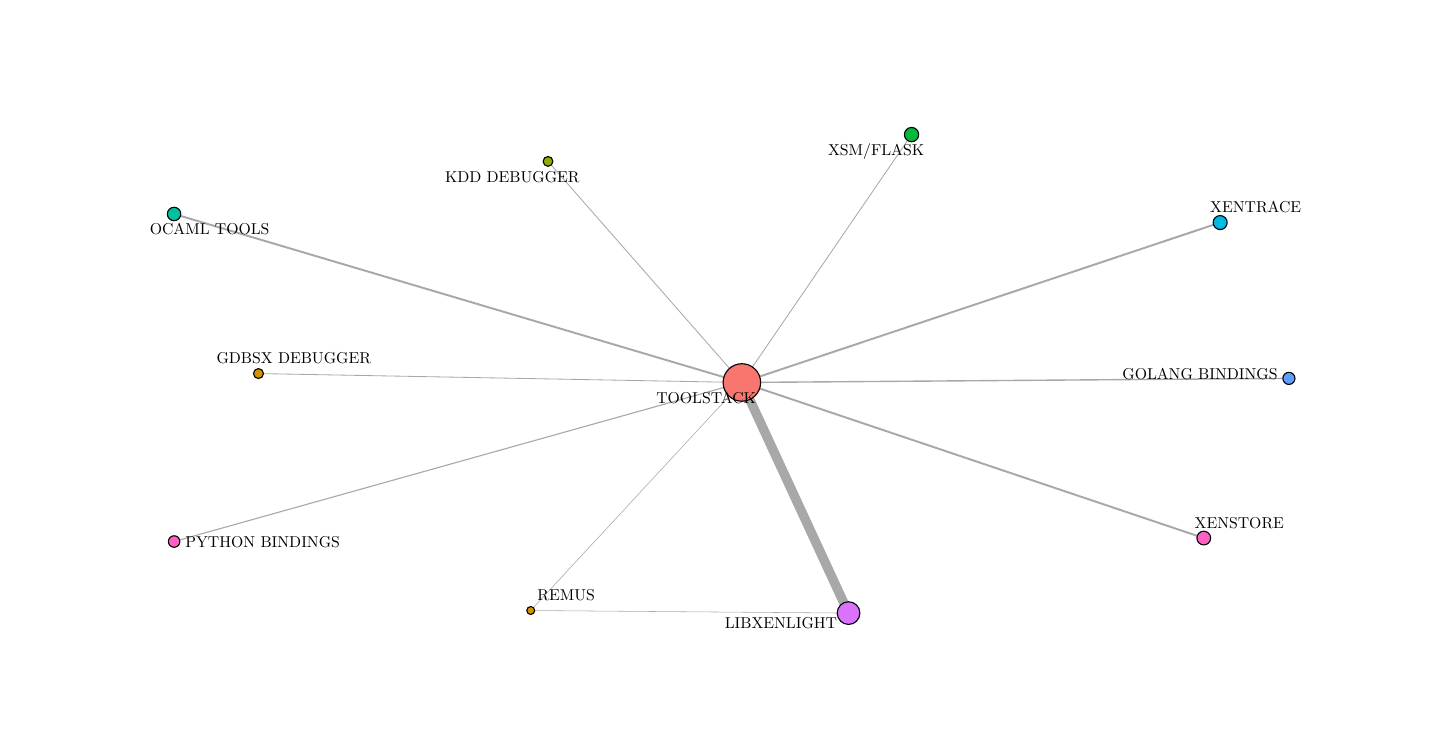
\begin{tikzpicture}[x=1pt,y=1pt]
\definecolor{fillColor}{RGB}{255,255,255}
\path[use as bounding box,fill=fillColor,fill opacity=0.00] (0,0) rectangle (505.89,252.94);
\begin{scope}
\path[clip] (  0.00,  0.00) rectangle (505.89,252.94);
\definecolor{fillColor}{RGB}{255,255,255}

\path[fill=fillColor] (  0.00,  0.00) rectangle (505.89,252.94);
\end{scope}
\begin{scope}
\path[clip] ( 32.75, 32.75) rectangle (475.89,222.94);
\definecolor{drawColor}{gray}{0.66}

\path[draw=drawColor,line width= 0.3pt,line join=round] ( 83.40,127.95) -- (258.07,124.73);

\path[draw=drawColor,line width= 0.5pt,line join=round] (455.75,126.21) -- (258.07,124.73);

\path[draw=drawColor,line width= 0.3pt,line join=round] (188.02,204.62) -- (258.07,124.73);

\path[draw=drawColor,line width= 0.2pt,line join=round] (296.62, 41.40) -- (181.77, 42.33);

\path[draw=drawColor,line width= 3.4pt,line join=round] (296.62, 41.40) -- (258.07,124.73);

\path[draw=drawColor,line width= 0.7pt,line join=round] ( 52.89,185.61) -- (258.07,124.73);

\path[draw=drawColor,line width= 0.4pt,line join=round] ( 52.92, 67.26) -- (258.07,124.73);

\path[draw=drawColor,line width= 0.2pt,line join=round] (181.77, 42.33) -- (258.07,124.73);

\path[draw=drawColor,line width= 0.7pt,line join=round] (258.07,124.73) -- (424.98, 68.51);

\path[draw=drawColor,line width= 0.7pt,line join=round] (258.07,124.73) -- (430.90,182.51);

\path[draw=drawColor,line width= 0.3pt,line join=round] (258.07,124.73) -- (319.39,214.30);
\definecolor{drawColor}{RGB}{0,0,0}
\definecolor{fillColor}{RGB}{211,146,0}

\path[draw=drawColor,line width= 0.4pt,line join=round,line cap=round,fill=fillColor] ( 83.40,127.95) circle (  1.80);
\definecolor{fillColor}{RGB}{97,156,255}

\path[draw=drawColor,line width= 0.4pt,line join=round,line cap=round,fill=fillColor] (455.75,126.21) circle (  2.19);
\definecolor{fillColor}{RGB}{147,170,0}

\path[draw=drawColor,line width= 0.4pt,line join=round,line cap=round,fill=fillColor] (188.02,204.62) circle (  1.77);
\definecolor{fillColor}{RGB}{219,114,251}

\path[draw=drawColor,line width= 0.4pt,line join=round,line cap=round,fill=fillColor] (296.62, 41.40) circle (  4.10);
\definecolor{fillColor}{RGB}{0,193,159}

\path[draw=drawColor,line width= 0.4pt,line join=round,line cap=round,fill=fillColor] ( 52.89,185.61) circle (  2.43);
\definecolor{fillColor}{RGB}{255,97,195}

\path[draw=drawColor,line width= 0.4pt,line join=round,line cap=round,fill=fillColor] ( 52.92, 67.26) circle (  2.08);
\definecolor{fillColor}{RGB}{211,146,0}

\path[draw=drawColor,line width= 0.4pt,line join=round,line cap=round,fill=fillColor] (181.77, 42.33) circle (  1.43);
\definecolor{fillColor}{RGB}{248,118,109}

\path[draw=drawColor,line width= 0.4pt,line join=round,line cap=round,fill=fillColor] (258.07,124.73) circle (  6.78);
\definecolor{fillColor}{RGB}{255,97,195}

\path[draw=drawColor,line width= 0.4pt,line join=round,line cap=round,fill=fillColor] (424.98, 68.51) circle (  2.48);
\definecolor{fillColor}{RGB}{0,185,227}

\path[draw=drawColor,line width= 0.4pt,line join=round,line cap=round,fill=fillColor] (430.90,182.51) circle (  2.53);
\definecolor{fillColor}{RGB}{0,186,56}

\path[draw=drawColor,line width= 0.4pt,line join=round,line cap=round,fill=fillColor] (319.39,214.30) circle (  2.58);

\node[text=drawColor,anchor=base,inner sep=0pt, outer sep=0pt, scale=  0.57] at ( 96.14,131.48) {GDBSX DEBUGGER};

\node[text=drawColor,anchor=base,inner sep=0pt, outer sep=0pt, scale=  0.57] at (423.62,125.85) {GOLANG BINDINGS};

\node[text=drawColor,anchor=base,inner sep=0pt, outer sep=0pt, scale=  0.57] at (175.13,197.12) {KDD DEBUGGER};

\node[text=drawColor,anchor=base,inner sep=0pt, outer sep=0pt, scale=  0.57] at (272.21, 35.78) {LIBXENLIGHT};

\node[text=drawColor,anchor=base,inner sep=0pt, outer sep=0pt, scale=  0.57] at ( 65.75,178.14) {OCAML TOOLS};

\node[text=drawColor,anchor=base,inner sep=0pt, outer sep=0pt, scale=  0.57] at ( 84.92, 64.92) {PYTHON BINDINGS};

\node[text=drawColor,anchor=base,inner sep=0pt, outer sep=0pt, scale=  0.57] at (194.59, 45.86) {REMUS};

\node[text=drawColor,anchor=base,inner sep=0pt, outer sep=0pt, scale=  0.57] at (245.17,117.26) {TOOLSTACK};

\node[text=drawColor,anchor=base,inner sep=0pt, outer sep=0pt, scale=  0.57] at (437.81, 72.05) {XENSTORE};

\node[text=drawColor,anchor=base,inner sep=0pt, outer sep=0pt, scale=  0.57] at (443.75,186.09) {XENTRACE};

\node[text=drawColor,anchor=base,inner sep=0pt, outer sep=0pt, scale=  0.57] at (306.57,206.85) {XSM/FLASK};
\end{scope}
\end{tikzpicture}
